\chapter{Introduction}\label{ch:intro}

In large-scale \ac{wifi} environments such as office buildings, shopping malls, and airports, where multiple \acp{ap} are required, people often move around indoors with their mobile devices.
To maintain a stable connection to the \ac{ssid}, the station must remain in the range of the \ac{ap} or may roam to another \ac{ap} with the same \ac{ssid}.
However, the current already improved roaming process in 802.11k/r\cite{802.11k}\cite{802.11r} does not consider human movement.
For example, if a user's station is moving away from \ac{ap}1 towards \ac{ap}2 and further towards \ac{ap}3, as seen in \Cref{fig:roaming}.
There is no initiation of a roam from \ac{ap}1 to \ac{ap}3, but instead the station will first roam from \ac{ap}1 to \ac{ap}2 and then to \ac{ap}3, which increases the number of roamings.

\begin{figure}[h]
    \centering
    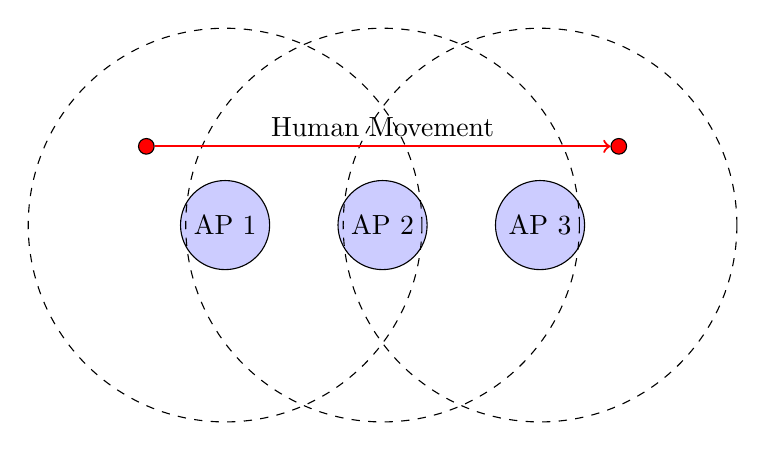
\begin{tikzpicture}
% Access Points
\node[draw, circle, fill=blue!20, minimum size=1cm] (ap1) at (0,0) {AP 1};
\node[draw, circle, fill=blue!20, minimum size=1cm] (ap2) at (2,0) {AP 2};
\node[draw, circle, fill=blue!20, minimum size=1cm] (ap3) at (4,0) {AP 3};

% Ranges
\draw[dashed] (ap1) circle (2.5cm);
\draw[dashed] (ap2) circle (2.5cm);
\draw[dashed] (ap3) circle (2.5cm);

% Person's movement
\node[draw, circle, fill=red, inner sep=2pt] (start) at (-1,1) {};
\node[draw, circle, fill=red, inner sep=2pt] (end) at (5,1) {};
\draw[->, thick, red] (start) -- (end) node[midway, above, black] {Human Movement};
\end{tikzpicture}
    \caption{Roaming process of a user's station from \ac{ap}1 to \ac{ap}3 bypassing also \ac{ap}2.}
    \label{fig:roaming}
\end{figure}

Real time applications such as video conferencing are particularly sensitive to these hand-offs, which may result in dropped connections and unsatisfied users.
Instead, it would be ideal if the movement from \ac{ap}1 to \ac{ap}3 was detected by the station beforehand and a roam from \ac{ap}1 to \ac{ap}3 was initiated.

Therefore, this thesis will explore if a time series \ac{ml} model can predict the nearest \ac{ap} a station may connect to next.
Because of the many \acp{ap} in large-scale \ac{wifi} environments, this prediction is a multi-class classification problem with many classes.
This leads to a hard prediction task, as the model needs to predict the next \ac{ap} out of many \acp{ap}.
To make the prediction task easier, the model will predict the top 3 \acp{ap} the station may connect to next.
So the nearest station needs to be in the top 3 of the predictions to be considered a correct prediction.
This prediction will be compared to a heuristic approach, which will choose the next \ac{ap} based on the last measured \ac{rssi} value.

A time series \ac{ml} model requires time series data as input.
There are two possible data sources: generate new or utilize existing data. 
Data generation needs a comprehensive plan for accounting data setup and collection.
As this process is time-consuming and needs a lot of planning and evaluation beforehand, this thesis will not generate data.
Thus, this thesis will use a pre-existing dataset with sensor data such as acceleration, waypoint data and \ac{wifi} data from large-scale environments.
The only dataset which is available with these requirements is from a 2021 competition by Microsoft Research \cite{IndoorLocationNavigation} on kaggle \cite{kaggle}.
The data will be analyzed in \Cref{ch:data-ana} to determine what parts of the data I will use for the \ac{ml} model.

After that, I will discuss the suitability of some pre-selected time series \ac{ml} models for the task in \Cref{ch:discuss-ml}. 
Because of findings in \Cref{ch:data-ana}, this thesis needs to preprocess the prepared data further and will implement the \ac{lstm} model for one site and floor of the competition in \Cref{ch:implementation}.
Finally, in \Cref{ch:evaluation}, I will evaluate the model's performance and, in \Cref{ch:conclusion}, conclude if this prediction could be useful in the future.
